\documentclass[12pt,twocolumn,letterpaper]{extarticle}


\setlength{\textheight}{9.075in}
\setlength{\textwidth}{7.075in}
\setlength{\columnsep}{0.3125in}
\setlength{\topmargin}{-0.3in}
\setlength{\headheight}{0in}
\setlength{\headsep}{0in}
\setlength{\parindent}{1pc}
\setlength{\oddsidemargin}{-.304in}
\setlength{\evensidemargin}{-.304in}

\usepackage{titlesec}
\usepackage{graphicx}
\usepackage{multicol}
\usepackage{subfigure}

% set section font size to 14pt
\titleformat{\section}{\fontsize{18}{20}\selectfont\bfseries}{\thesection}{1em}{}

% set subsection font size to 12pt
\titleformat{\subsection}{\fontsize{14}{16}\selectfont\bfseries}{\thesubsection}{1em}{}


\usepackage{times}
\usepackage{epsfig}
\usepackage{graphicx}
\usepackage{amsmath}
\usepackage{amssymb}
\usepackage{courier}
\usepackage{multirow}
\usepackage[svgnames]{xcolor}
\usepackage{tabularx}
\usepackage{booktabs,chemformula}
\usepackage{float}

\usepackage[colorlinks=true, allcolors=blue]{hyperref}

\setcounter{page}{1}
\begin{document}

\title{Optimization for Deep Learning Final Project: \\
A study on autodiff in PyTorch}
\author{
  Hsiu-Hsuan Wang\thanks{The main author of this paper} \\
  \texttt{b09902033@ntu.edu.tw}
  \and
  Yu-Kai Hung \\
  \texttt{b09902040@ntu.edu.tw}
}
\date{}
\maketitle

\section*{Abstract}

Automatic differentiation is a core implementation of a deep learning library. An efficient and straight-forward implementation of automatic differentiation is the key factor for fast and productive development of deep learning research. Recently, PyTorch and TensorFlow are the two dominant deep learning library. However, their implementation and design of automatic differentiation differ significantly due to various practical considerations. This motivate us to conduct detailed investigation in their implementation. We explain the difference between static graph and dynamic graph\;(eager execution) in both library along with the motivations and considerations behind them. We also provide extensive experiments and analyses for various of scenarios. Our work aims to offer valuable insights and practical recommendations for future studies on automatic differentiation within the research community. By providing directions and suggestions, we hope to foster advancements in this field and contribute to its ongoing development.

\section{Introduction}

Computing the differentiation is a fundamental component to gradient descent optimization. Some methods include \emph{numerical differentiation}, \emph{symbolic differentiation}, and \emph{automatic differentiation} are the main approaches that are widely implemented in deep learning libraries, including Chainer \cite{tokui2015chainer}, PyTorch \cite{NEURIPS2019_bdbca288}, TensorFlow \cite{45381}, etc. However, due to the implicit definition and computation of automatic differentiation\;(autodiff), it becomes non-trivial to trace the implementation of the backpropagation in a network. PyTorch library is designed for rapidly developing the deep learning research, which is the main motivation for it to utilize define-by-run computation graph and run in eager execution \cite{paszke2017automatic}. 

As the differentiation process is handled automatically, one can use straight forward programming to design any complicated networks. Therefore, we are curious about the hidden computation process and performance about the PyTorch library. In this work, we delve into the mechanics of autodiff in PyTorch and compare the execution time of backward gradient flow with the TensorFlow library, a competitive deep learning library to PyTorch. We also conduct extensive experiment to analyze the potential factor and optimization to try to give practical suggestions under different scenario. These two library use different execution design for autodiff. TensorFlow 1.0 implements static computation graph, which allow its model to be compiled and optimized to run faster. In contrast, TensorFlow 2.0 runs tensor computation in eager mode, which is same as PyTorch library. Eager execution does not explicitly implement the tape, but dynamically generate the computation graph, which allow more flexible and dynamic model structure (e.g.\ sequence-to-sequence model). On top of that, PyTorch and TensorFlow 2.0 also support the static computation graph, in which the model would be compiled and optimized to improve performance and portability. We organize our contribution in the following order. In Section~\ref{sec:problem-definition}, we would define both eager execution and graph execution and our hypothesis for the experiment. In Section~\ref{sec-experiment}, we conduct extensive experiments to describe the implementation details of autodiff in PyTorch and TensorFlow. In Section~\ref{sec-conclusion}, we point out the limitation of our work along with some future direction for the community to study autodiff and its implementation.

\section{Problem Definition} \label{sec:problem-definition}

\subsection{Autodiff in PyTorch}

According to \cite{paszke2017automatic}, PyTorch supports reversed-mode automatic differentiation (autodiff) and the implementation is \emph{dynamic}\;(define-by-run execution) and \emph{immediate}\;(eager execution). The dynamic design allows user to use common coding syntax to define the computation of function, then the computation graph would be dynamically built. The eager execution would execute the computation immediately, instead of waiting the whole forward graph being built. Hence, the autodiff is \emph{tape-free}, which means that each function would only records the subgraph with essential results of differentiation. This design prevent the explicit synchronization among the whole computation graph. In this way, the execution can be accelerated by pipeline CPU and GPU.

Nonetheless, there are some drawbacks for this tape-free design, including the optimization and batching limitation of the whole network, the unavoidable overhead to rebuild the forwards and backwards graph in every iteration. To solve these potential issues, PyTorch utilizes the carefully tuned C++ library as a compensate for the efficiency. In conclusion, PyTorch can actually obtain superious throughput results among other tensor computation framework \cite{NEURIPS2019_bdbca288}.

Besides eager execution, PyTorch implements JIT\;(Just-In-Time) library that support \texttt{trace} or \texttt{script} function to compile and optimize the PyTorch function and model. We also observe such performance improvement in our experiment \ref{sec-experiment}.

\subsection{Autodiff in Tensorflow} \label{sec:tensorflow}

TensorFlow provide two modes: \emph{static graph}\; (graph mode) and \emph{eager execution}. In graph mode, the computation graph is built before training and persistent in the whole training process. Since the graph is built before running-time, its structure can be further optimized during compiling and distributed to multiple devices to achieve parallel acceleration. However, one of the disadvantages of this static design is that the compiled execution object is hard to debugging during development. On top of that, the size of tensors in each operation should be fixed, which is inconvenience to implement models with various input or output length (e.g. RNN). Practically, one can wrap any custom function with TensorFlow computation with the \texttt{@tf.function} decorator to speed up the computation by running in graph mode instead of eager mode.

As for \emph{eager execution}, it evaluates and runs each computation immediately, which is easy for debugging and fit for flexible size of tensors. Also, the natural control flow can be used as how Python usually do, makes it easy to developing the training script for various type of models. 

\subsection{Backpropagation in Deep Learning}
In the training phrase of deep learning models, a computation graph would be build to store the operators and variable and output the resuls. This process is defined as \emph{forward pass}. Afterward, the model would compute the training loss using a loss function that measures the correctness of the output. The gradient of the loss, as the guidance of the model, would flow backward to update all the model parameters.

\section{Experiments} \label{sec-experiment}

Since both PyTorch and TensorFlow has eager mode, we take advantage of them to synchronize the configuration on both script to make our experiment fair. Intuitively, the backward process of Tensorflow in graph mode should be faster than the default eager executing PyTorch since the models in Tensorflow are compiled before running. Therefore, we conduct experiments to verify whether the above assumption holds empirically. In Section~\ref{sec:exp-1}, we measure the execution time of the multi-layer perceptron and provide various analysis to support our experiment results. In Section~\ref{exp-2}, we measure the running time of several famous basic models including convolution layer, fully-connected layer and long-short term memory layer.

\subsection{Compute Gradients of MLP} \label{sec:exp-1}

In this experiment, we compare the execution time of backward pass in multi-layer perceptron\;(MLP) between TensorFlow and PyTorch framework. These two frameworks both support eager execution and graph execution, where eager execution run the tensor computation on-the-fly while the graph execution would compile and optimize the whole model. We provide the results of eager execution mode in Sec~\ref{par:eager} and graph execution in Sec~\ref{par:graph}. As mentioned in Sec~\ref{sec:tensorflow}, Tensorflow provide eager execution in its 2.0 version as default mode. On the contrary, PyTorch implements dynamic eager execution with virtually no sacrifice in performance \cite{NEURIPS2019_bdbca288}.

\subsubsection{Experiment Setup}
We implement a simple MLP in both TensorFlow and PyTorch to ensure that they perform identical computation in forward pass. The  $i$th MLP layer is composed of a projection matrix $W_i$, a bias term $b_i$ and a ReLU activation function. The explicit formulation is provided in Eq~\ref{eq:MLP_layer} where $Z^l$ is the input of the $l$th layer.
\begin{equation} \label{eq:MLP_layer}
    Z^{l+1} = \max\left(0, W_i Z^{l} + b_i\right)
\end{equation}
The initial results show that the mean difference between the gradient of PyTorch and TensorFlow is less than $10^{-5}$, which guarantee the correctness of our implementation under both framework.

We simulate the full MNIST dataset to run the experiment. Specifically, we generate 60000 input instance with $784$ dimension to measure the execution time of an epoch of data. The synthetic dataset is desined identical to the MNIST dataset \cite{deng2012mnist}. The batch size is set to 128, so there would be 469 backward pass in one experiments.

\subsubsection{Eager execution} \label{par:eager}

Both PyTorch and TensorFlow would run with eager execution by default. The exact codes is provided in Fig~\ref{fig:pytorch-eager} and \ref{fig:tensorflow-eager}.

\begin{figure}[ht]
    \centering
    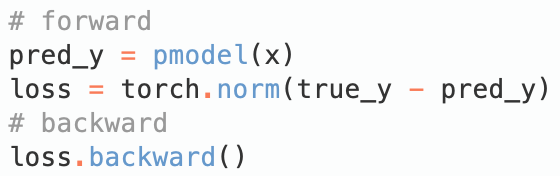
\includegraphics[width=0.8\columnwidth]{images/pytorch-eager.png}
    \caption{The python code of PyTorch's forward and backward pass. The codes for measuring the execution time have been removed.}
    \label{fig:pytorch-eager}
\end{figure}

\begin{figure}[ht]
    \centering
    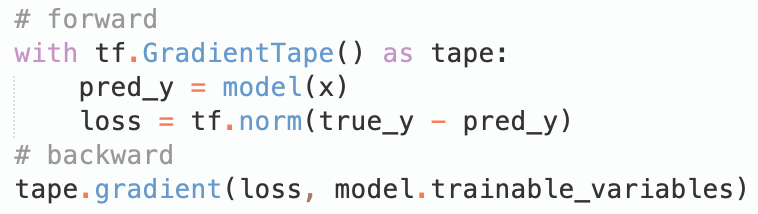
\includegraphics[width=0.8\columnwidth]{images/tensorflow-eager.png}
    \caption{The python code of TensorFlow's forward and backward pass. The codes for measuring the execution time have been removed.}
    \label{fig:tensorflow-eager}
\end{figure}

We provide the mean average and standard deviation of the execution time for five trials in Table~\ref{tab:exp-1-eager}. The execution time of the backward pass increase when the MLP becomes deeper, while the total number of model parameters is similar. That is, the depth of MLP is one factor that impact the execution time of backward pass.

\begin{table*}[t]
    \centering
    \caption{Experiment results in \emph{eager} mode. The execution time is measured in $\mu s$. The same experiment is run for five trials and the mean and std is reported.}\label{tab:exp-1-eager}
    \vskip 0.1in
    \resizebox{0.7\textwidth}{!}{%
        \begin{tabular}{cc|cccc}
        \toprule
        \multirow{2}{*}{Hidden layer shape} & \multirow{2}{*}{\# model parameters} & \multicolumn{2}{c}{PyTorch} & \multicolumn{2}{c}{TensorFlow} \\ 
        & & mean & std & mean & std \\
        \midrule
        $[512]$ & 406528 & 686$\pm$21 & 68$\pm$6 & 2889$\pm$49 & 212$\pm$8 \\
        $[354, 354]$ & 406392 & 949$\pm$16 & 78$\pm$12 & 4515$\pm$49 & 264$\pm$52 \\
        $[294, 294, 294]$ & 406308 & 1162$\pm$20 & 76$\pm$2 & 5718$\pm$37 & 207$\pm$19 \\
        \bottomrule
        \end{tabular}%
    }
\end{table*}

\subsubsection{Graph execution} \label{par:graph}

As mentioned in \ref{sec:problem-definition}, one can execute a function in graph mode by adding the decorator \texttt{@tf.function}. The function would then been compiled and optimized for faster execution time. Similarly, PyTorch also provide \texttt{script} function wrapper to achieve similar acceleration by compiling the model. In this experiment, we conduct the exact same experiment as in Sec~\ref{par:eager}, and show the results in Table.

\begin{table*}[t]
    \centering
    \caption{Experiment results in \emph{graph} mode. The execution time is measured in $\mu s$. The same experiment is run for five trials and the mean and std is reported. The improvement column represents the degree of improvement when transitioning from eager mode to graph (script) mode.}\label{tab:exp-1-graph}
    \vskip 0.1in
    \resizebox{0.7\textwidth}{!}{%
        \begin{tabular}{c|ccc|ccc}
        \toprule
        \multirow{2}{*}{MLP Structure} & \multicolumn{3}{c}{PyTorch} & \multicolumn{3}{c}{TensorFlow} \\ 
        & mean & std & improvement($\uparrow$) & mean & std & improvement($\uparrow$) \\
        \midrule
        $[512]$ & 465$\pm$14 & 21$\pm$18 & 1.47 & 538$\pm$55 & 106$\pm$38 & 5.36 \\
        $[354, 354]$ & 720$\pm$4 & 47$\pm$54 & 1.31 & 1247$\pm$97 & 339$\pm$64 & 3.62 \\
        $[294, 294, 294]$ & 900$\pm$3 & 38$\pm$35 & 1.29 & 1581$\pm$173 & 331$\pm$198 & 3.61 \\
        \bottomrule
        \end{tabular}%
    }
\end{table*}

\paragraph{Large initial execution time} It is worth noting that we observe some large execution time (approximately 50x compare to the other batches) in the first batch of TensorFlow's graph mode execution. The similar pattern is also observed in PyTorch's scripted model. The second, third, and fourth batch would also take $\sim 50$ more time to execute compare the the other batches. The observed pattern is visualized in Fig~\ref{fig:large-init}. Since we only discover these outlier batch in the compiled model, we can conclude that these models have done some initialization or loading when they are called in the first time. We leave the deeper investigation as the future work.

\begin{figure}[htbp]
  \centering
  \begin{subfigure}
    \centering
    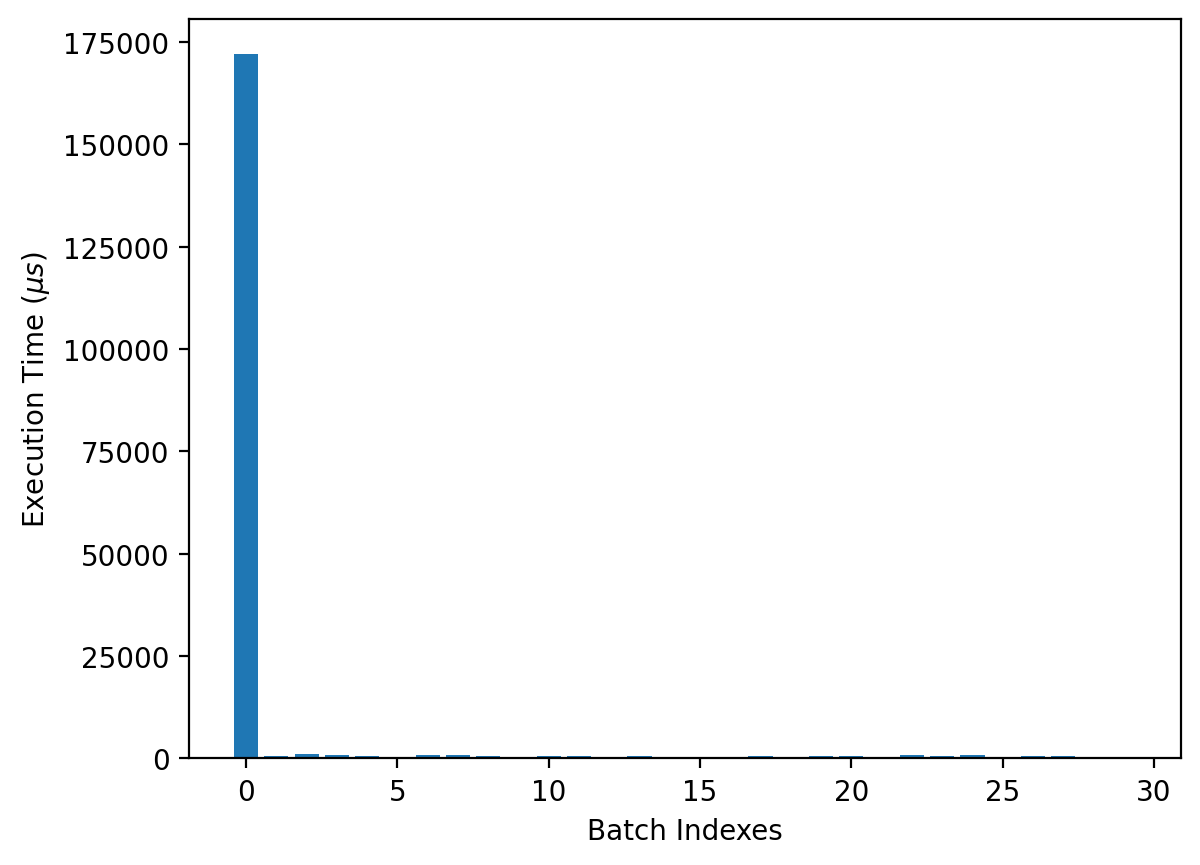
\includegraphics[width=0.45\columnwidth]{images/tf-graph.png}
  \end{subfigure}
  \hfill
  \begin{subfigure}
    \centering
    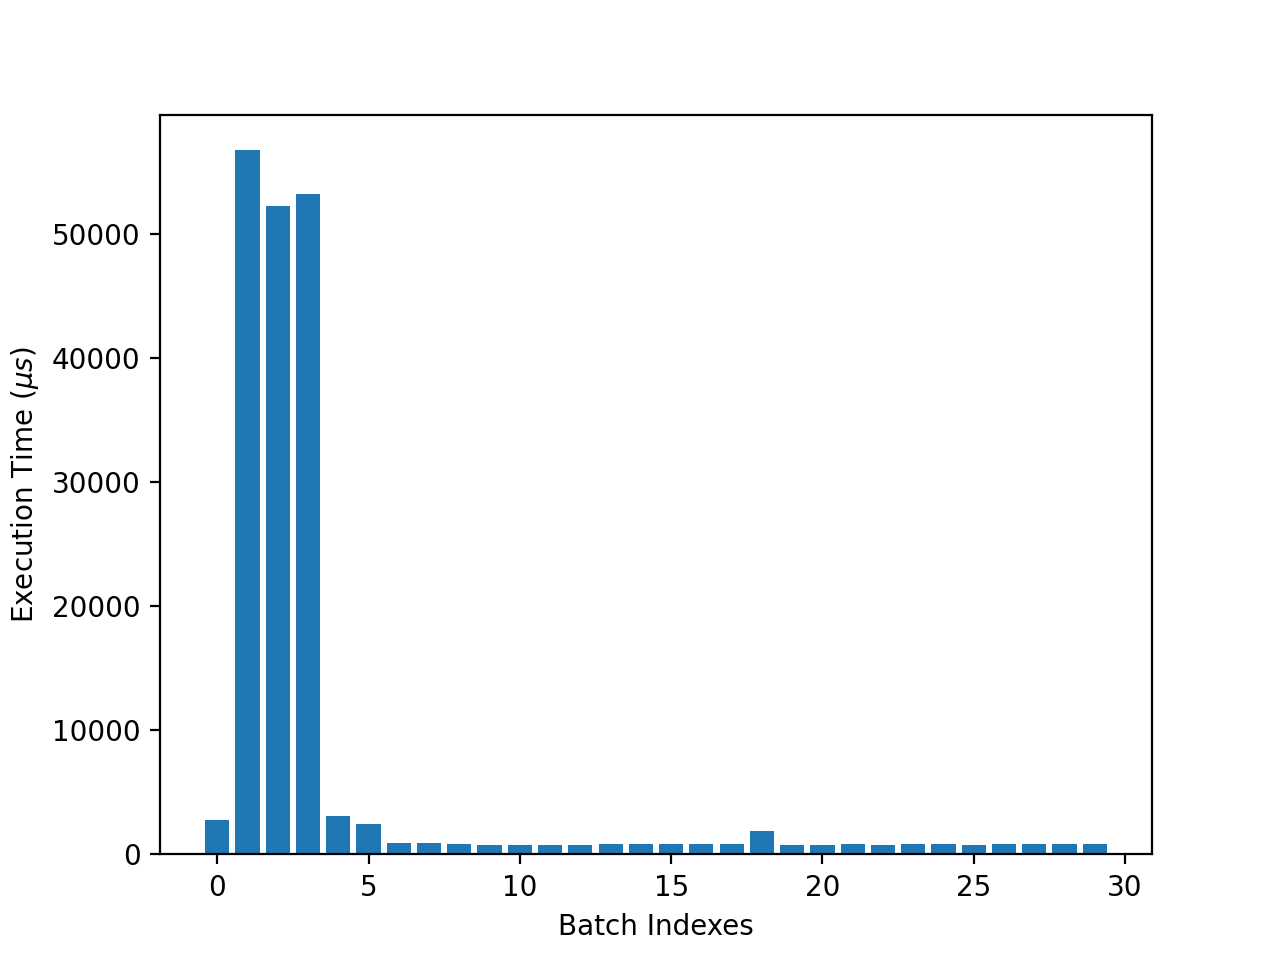
\includegraphics[width=0.47\columnwidth]{images/pt-script.png}
  \end{subfigure}

  \caption{The visualization of large initial execution time observed in TensorFlow function in graph mode(\textbf{left}) and scripted PyTorch model(\textbf{right})}.
  \label{fig:large-init}
\end{figure}

\subsubsection{Computation Graph Analysis}

Since the computation graph is dynamic and define-by-run, it is hard to investigate the implicit backward function. One efficient tool to understand the whole forward and backward function is the visualization of computation graph. In fact, both PyTorch and TensorFlow has the relevant package to display the computation graph.

\paragraph{Computation graph of PyTorch}

The torchviz\footnote{\url{https://github.com/szagoruyko/pytorchviz}} library provides functions to visualize the computation graph in great detail. The generated computation graph is shown in Fig~\ref{fig:pt-computation-graph}. The blue blocks represent the reachable tensor from the model that requires grad. The orange blocks are the saved information for the model to conduct the autodiff when the \texttt{backward} function is called. The green blocks are the output of the model. In the 512-MLP model, we compute two matrix-matrix product and two vector addition operations, as well as one subtraction and one vector normalization in the loss function. All of these operations has their backward\;(differential) function defined in gray. The \texttt{AccumulatedGrad} node would accumulate all the incoming gradient for the leaf nodes colored in blue. With the visualization, we can have a clear understanding about the implicit backward process of autodiff in PyTorch.

\begin{figure}[ht]
    \centering
    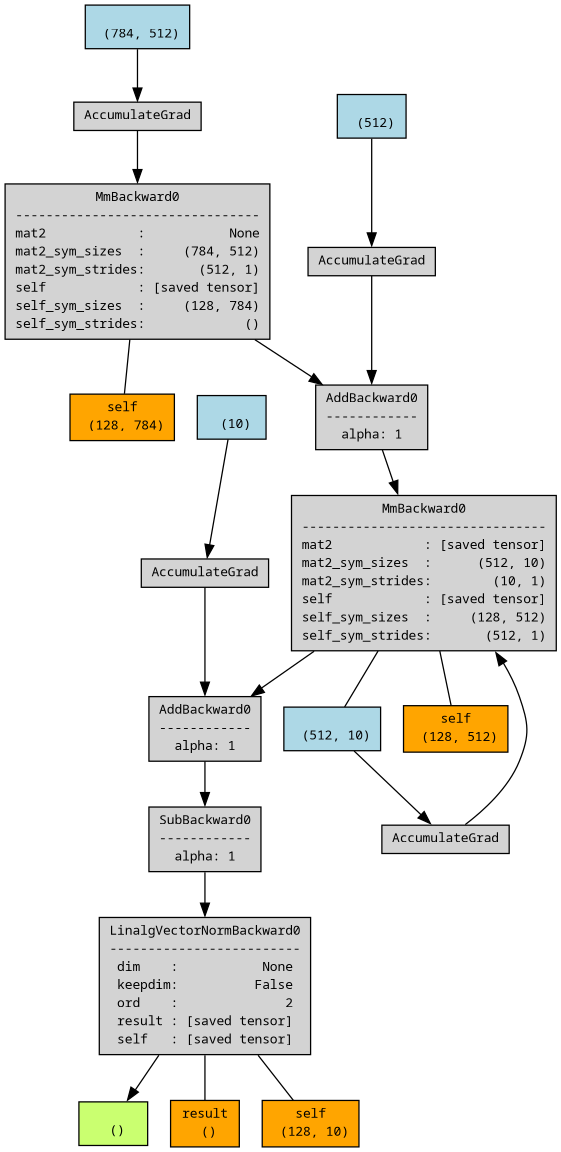
\includegraphics[width=0.8\columnwidth]{images/pt-computation-graph.png}
    \caption{The computation graph of the 512-MLP model generated by \texttt{torchviz} library.}
    \label{fig:pt-computation-graph}
\end{figure}

\paragraph{Computation graph of TensorFlow}

The official TensorFlow library already provides functions\footnote{\url{https://www.tensorflow.org/tensorboard/graphs}} to visualize the computation graph. The generated computation graph is shown in Fig, however, does not provide clear documentation about each component. Even though the TensorFlow library support various approaches to generate the graph, the function usages are actually confusing. Since TensorFlow 1.0 only supports static graph, whereas TensorFlow 2.0 supports both static graph and eager execution, the library structure changes a lot without clear documentation.

Based on the aforementioned reasons, we can only provide non-rigorous definitions of the components. \texttt{tf\_x} is the input data feature of the 512-MLP network. \texttt{true\_y} would be used to compute the loss along with the output of \texttt{tf\_linear\_6}. The \texttt{gradient\_tape} is a subnode that records the same computation graph containing both \texttt{norm} and \texttt{tf\_linear\_6}. This matches the designed usage of the \texttt{gradient\_tape} component as it is used to record all the computation. The \texttt{identity}, \texttt{identity\_1}, \texttt{identity\_2}, and \texttt{identity\_3} are the four gradient for the two projection matrices and biases in the 512-MLP. To conclude, the clear documentation is needed for others to further understand the computation graph generated by TensorFlow.

\begin{figure}[ht]
    \centering
    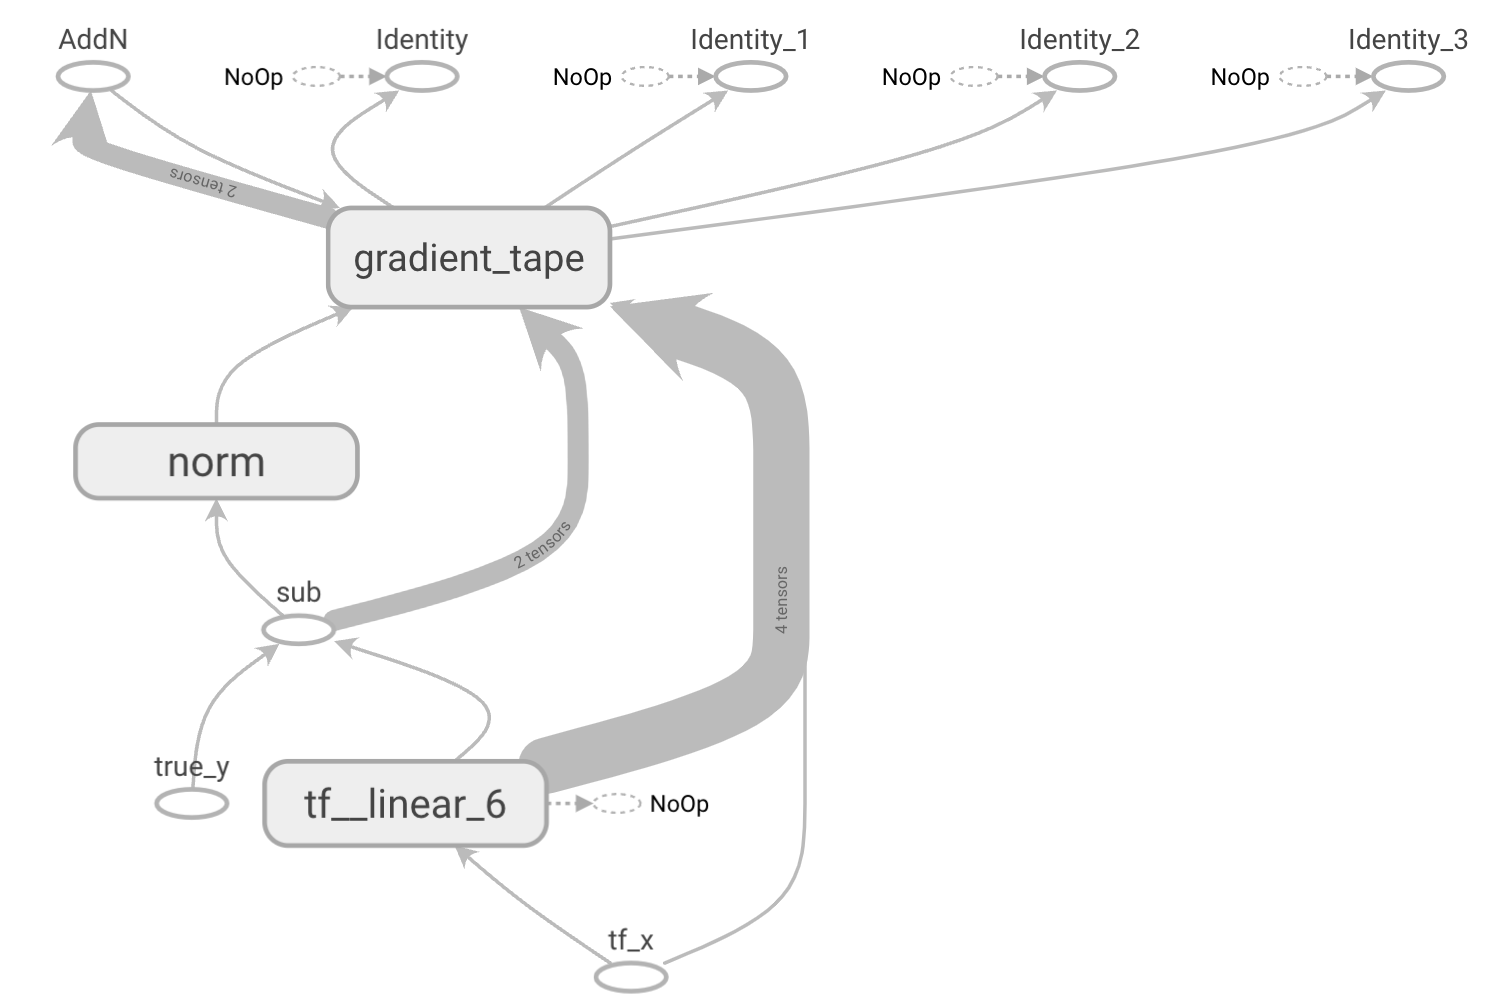
\includegraphics[width=0.8\columnwidth]{images/tf-computation-graph.png}
    \caption{The computation graph of the 512-MLP model generated by the official TensorFlow library.}
    \label{fig:pt-computation-graph}
\end{figure}

\subsection{Compute the Jacobian of Different Layers} \label{exp-2}

It is worth noting that we have to wrap the Jacobian function of Tensorflow with the \texttt{@tf.function} decorator to speed up the computation by running in graph mode. The results are in Table~\ref{tab:exp-1}

Our experiment is done in "linux4" with single thread of CPU.

As we can see, The running time of TensorFlow (eager) in Fully Connected Network is similar to PyTorch. This proved our Hypo 0.
Another thing to notice is the running time of graph mode. We expected it is the lowest one with the help of graph optimization. We think it is because of the single core CPU affecting the parallel performance and the tiny basic network structures with limited optimization possibilities. Thus, we made another assumption: when working on larger models (e.g. ResNet) in these modes, the Tensorflow (graph) can do much better than the others. 

To prove our assumption, we made another experiment with ResNet50 and attached the result in Table 4. We can see an incredible strength of graph mode when there are lots of optimization possibilities of large model, the amount of time that can be saved through forehead-built graph.

Finally, we can conclude that if we want to start another Deep Learning research, we could choose PyTorch (naive) because of their flexibility, convenient debugging properties and great performance on small structure of neural network. When dealing the larger model and training in the long run, TensorFlow (Graph Mode) is the best choice!

\begin{table}[t]
    \centering
    \caption{Experiment results.}\label{tab:exp-1}
    \resizebox{\columnwidth}{!}{%
    \begin{tabular}{llll}
    \toprule
    Runtime / STD ($10^{-5}$s) & FCN & CNN & LSTM  \\ 
    \midrule
    Tensorflow (graph) & 216 / 15 & 91 / 7 & 98 / 20 \\
    Tensorflow (eager) & 249 / 25 & \textbf{11698} / 1079 & \textbf{23031} / 2034\\
    PyTorch (naive) & 258 / 60 & 225 / 27 & 529 / 50\\
    PyTorch (script) & \textbf{1167} / 60 & 272 / 50 & 574 / 52\\
    
    \bottomrule
    \end{tabular}%
    }
\end{table}


\begin{table}[t]
    \centering
    \caption{Experiment results.}\label{tab:exp-1}
    \resizebox{\columnwidth}{!}{%
    \begin{tabular}{ll}
    \toprule
    Runtime / STD (s) & ResNet50  \\ 
    \midrule
    Tensorflow (eager) & 11.179 / 0.3152 \\
    Tensorflow (graph) & 0.9339 / 0.1104 \\
    PyTorch (script) & 45.0729 / 0.6323 \\
    PyTorch (naive) & 44.8822 / 0.4035 \\
    \bottomrule
    \end{tabular}%
    }
\end{table}

\section{Conclusion} \label{sec-conclusion}

We prove that the backward computation can be faster when running in a static graph. Our experiment results show that PyTorch can run faster in small model, while the TensorFlow model runs faster than PyTorch in larger model under graph mode. However, our work did not explore the execution time on GPU, while both PyTorch and TensorFlow can reach their best parallel execution on it. Our work provide some analysis results and directions for more future study to investigate border and deeper about the empirical performance of the autodiff in libraries beyond PyTorch and TensorFlow.

\newpage
\clearpage
\bibliographystyle{plain}
\bibliography{ref}


\end{document}
%%% Local Variables:
%%% mode: latex
%%% TeX-master: t
%%% End: